\chapter{Capa Motivacional}
\label{chap:Motivacional}
\textit{En el aparte se describe el desarrollo de la Arquitectura Empresarial\index{Arquitectura Empresarial} correspondiente a la Capa Motivacional utilizando Archimate\index{Archimate}.}
\vspace{2ex}\vfill
\minitoc
\cleardoublepage

\section{Punto de Vista de Stakeholder\index{Stakeholder}}
El punto de vista de stakeholders nos permite al analizar para modelar las partes interesadas o implicados, los manejadores internos y externos para el cambio, y se efectúan evaluaciones (en términos de fortalezas, debilidades, oportunidades y amenazas) de estos manejadores. Los objetivos constituyen la base para el proceso de ingeniería de requisitos, incluyendo el refinamiento meta, contribución y análisis de conflictos. \cite{ref9}
    
  \begin{table}[H]
  	\centering
   	\begin{tabular}{p{3.7cm}p{8cm}}
   		\hline
   		\rowcolor[HTML]{0073a1}
   		{\color[HTML]{FFFFFF} \textbf{Nombre}} & {\color[HTML]{FFFFFF} \textbf{Vista de Stakeholder\index{Stakeholder}}} \\
   		\hline
   		\textbf{Stakeholder\index{Stakeholder}s} & Stakeholder\index{Stakeholder}s, administradores de empresas, arquitectos TIC\index{TIC}, analistas de negocios, Analistas de requerimientos \\
   		\textbf{Preocupaciones} & Misión de la arquitectura y la estrategia, motivación \\
   		\textbf{Propósito} & Diseñar\index{Diseñar}, decidir, informar \\
   		\textbf{Nivel de Abstracción\index{Abstracción}} & Coherencia\index{Coherencia}, detalle \\
   		\textbf{Capa} & Capa de Negocio\index{Negocio}s, Aplicación\index{Aplicación} y tecnología \\
   		\textbf{Aspectos} & Motivación \\
   		\bottomrule
   	\end{tabular}
   	\captionsetup{width=.95\textwidth}
   	\caption{Descripción punto de vista de stakeholders \cite{ref9}}
   	\label{tabla20}
  \end{table}
    
  \begin{figure}[H]
   	\centering
   	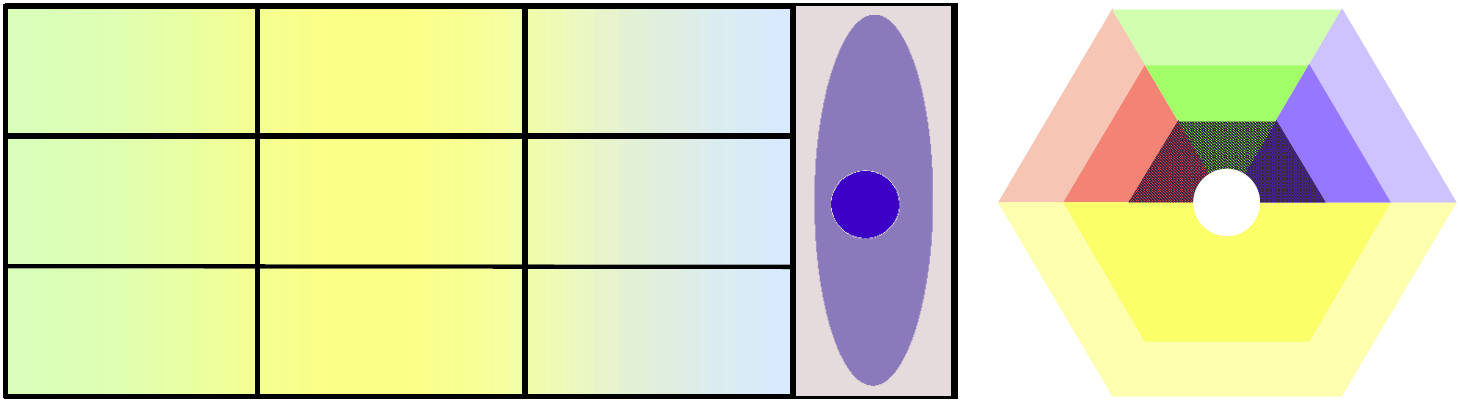
\includegraphics[scale=0.2]{figuras/29}
   	\captionsetup{width=.95\textwidth}
   	\caption{Posición del punto de vista de stakeholders conceptualmente y marco del punto de vista \cite{ref9}}
   	\label{figura29}
   \end{figure}
   
   \subsection{Metamodelo\index{Metamodelo}}
   En la Figura \ref{metamodelo17} se ilustra el metamodelo del punto de vista de Stakeholder\index{Stakeholder} donde el pivote de todo es el objetivo, por medio del cual se establece la relación entre los stakeholders, los manejadores y la valoración o apreciaciones generadas desde los objetivos que le apuntan a situaciones propositivas para la organización; se hace énfasis en como los stakeholders juegan con los objetivos de la organización. \cite{ref9}
   
   \begin{figure}[H]
   	\centering
   	\includegraphics{metamodelos/17}
   	\captionsetup{width=.95\textwidth}
   	\caption{Metamodelo\index{Metamodelo} punto de vista de stakeholders \cite{ref9}}
   	\label{metamodelo17}
   \end{figure}
   
   \subsection{Modelo mInstituto}
   Dentro del modelo de stakeholder tenemos como principales componentes el desarrollador quien sera el encargado de proveer las soluciones tecnológicas de la organización, para nuestro caso el aplicativo para instituciones minstituto. También tenemos la parte comercial con un objetivo principal que es generar el reconocimiento de nuestra empresa y sus productos para cada día obtener una mayor participación del mercado.
   
   \begin{figure}[H]
   	\centering
   	\includegraphics[scale=0.7]{modelos/17}
   	\captionsetup{width=.95\textwidth}
   	\caption{Modelo punto de vista de stakeholders: minstituto}
   	\label{modelo17}
   \end{figure}
   
\section{Punto de Vista de Realización de Objetivos}
El punto de vista de la realización de objetivos permite a un diseñador modelar y refinar los objetivos (de alto nivel) en objetivos más concretos, y el refinamiento de objetivos concretos en requisitos o limitaciones que describen las propiedades que se necesitan para alcanzar los objetivos. El refinamiento de objetivos en sub objetivos se modela utilizando la relación de agregación. El refinamiento de objetivos en los requisitos se modela utilizando la relación realización. \cite{ref9}
      
   \begin{table}[H]
   	\centering
   	\begin{tabular}{p{3.7cm}p{8cm}}
   		\hline
   		\rowcolor[HTML]{0073a1}
   		{\color[HTML]{FFFFFF} \textbf{Nombre}} & {\color[HTML]{FFFFFF} \textbf{Realización de Objetivos}} \\
   		\hline
   		\textbf{Stakeholder\index{Stakeholder}s} & Stakeholder\index{Stakeholder}s, administradores de empresas, arquitectos TIC\index{TIC}, analistas de negocios, Analistas de requerimientos \\
   		\textbf{Preocupaciones} & Misión de arquitectura, estrategia y táctica, motivación \\
   		\textbf{Propósito} & Diseñar\index{Diseñar}, decidir \\
   		\textbf{Nivel de Abstracción\index{Abstracción}} & Coherencia\index{Coherencia}, detalle \\
   		\textbf{Capa} & Capa de negocio, tecnología \\
   		\textbf{Aspectos} & Motivación \\
   		\bottomrule
   	\end{tabular}
   	\captionsetup{width=.95\textwidth}
   	\caption{Descripción punto de vista de la realización de objetivos \cite{ref9}}
   	\label{tabla21}
   \end{table}
   
   \begin{figure}[H]
   	\centering
   	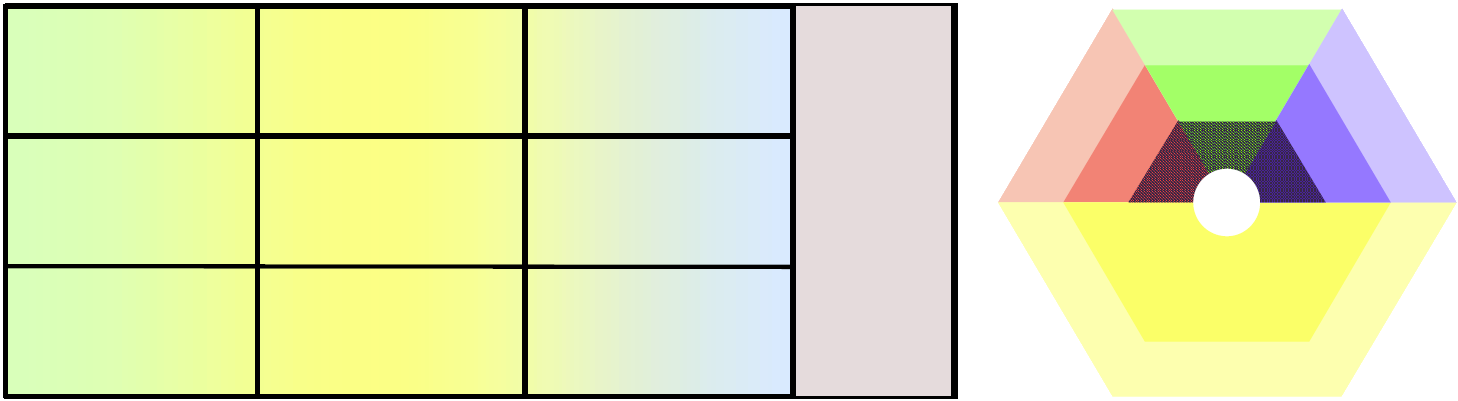
\includegraphics[scale=0.2]{figuras/30}
   	\captionsetup{width=.95\textwidth}
   	\caption{Posición del punto de vista de la realización de objetivos conceptualmente y marco del punto de vista \cite{ref9}}
   	\label{figura30}
   \end{figure}
   
   \subsection{Metamodelo\index{Metamodelo}}
   En la Figura \ref{metamodelo18} se ilustra el metamodelo del punto de vista de Realización de Objetivos, donde un objetivo se convierte en un requerimiento, el objetivo se realiza con un requerimiento o una restricción. \\
   
   Teniendo en cuenta que la restricción es un requerimiento pero lo diferencia porque tiene algún límite o alcance, el principio es un concepto para consolidar la arquitectura empresarial. \cite{ref9}
   
   \begin{figure}[H]
   	\centering
   	\includegraphics{metamodelos/18}
   	\captionsetup{width=.95\textwidth}
   	\caption{Metamodelo\index{Metamodelo} punto de vista de la realización de objetivos \cite{ref9}}
   	\label{metamodelo18}
   \end{figure}
   
   \subsection{Modelo mInstituto}
   Como principal objetivo de la organización tenemos proveer soluciones tecnológicas con un primer producto minstituto; cuya funcionalidad se basa en optimizar la gestión de la información en las instituciones educativas. Es importante resaltar que este no sera un desarrollo a la medida de cada cliente sino que manejaremos un paquete de funcionalidades comunes englobadas en unas licencias de uso estándar \\
   
   Otro de nuestros objetivos es que los productos software nos den el reconocimiento necesario en cada uno de los mercados a los que nos enfoquemos. Esto solo sera posible si tenemos clientes que puedan ser esos casos exitosos que podamos mostrar.

   \begin{figure}[H]
   	\centering
   	\includegraphics[scale=0.7]{modelos/18}
   	\captionsetup{width=.95\textwidth}
   	\caption{Modelo punto de vista de la realización de objetivos: minstituto}
   	\label{modelo18}
   \end{figure}
   
\section{Punto de Vista de Contribución}
El punto de vista de la contribución de objetivos permite a un diseñador o analista modelar las relaciones de influencia entre los objetivos y los requisitos. Los puntos de vista resultantes pueden utilizarse para analizar el impacto que las metas tienen para detectar conflictos entre los objetivos de las partes interesadas. La Tabla \ref{tabla22} describe el punto de vista. \cite{ref9}
   
   \begin{table}[H]
   	\centering
   	\begin{tabular}{p{3.7cm}p{8cm}}
   		\hline
   		\rowcolor[HTML]{0073a1}
   		{\color[HTML]{FFFFFF} \textbf{Nombre}} & {\color[HTML]{FFFFFF} \textbf{Vista de Contribución}} \\
   		\hline
   		\textbf{Stakeholder\index{Stakeholder}s} & Stakeholder\index{Stakeholder}s, administradores de empresas, arquitectos TIC\index{TIC}, analistas de negocios, Analistas de requerimientos \\
   		\textbf{Preocupaciones} &  Misión de arquitectura, estrategia y táctica, motivación \\
   		\textbf{Propósito} & Diseñar\index{Diseñar}, decidir \\
   		\textbf{Nivel de Abstracción\index{Abstracción}} & Coherencia\index{Coherencia}, detalle \\
   		\textbf{Capa} & Capa de negocio, Capa de tecnología \\
   		\textbf{Aspectos} & Motivación \\
   		\bottomrule
   	\end{tabular}
   	\captionsetup{width=.95\textwidth}
   	\caption{Descripción punto de vista de la contribución \cite{ref9}}
   	\label{tabla22}
   \end{table}
   
   \begin{figure}[H]
   	\centering
   	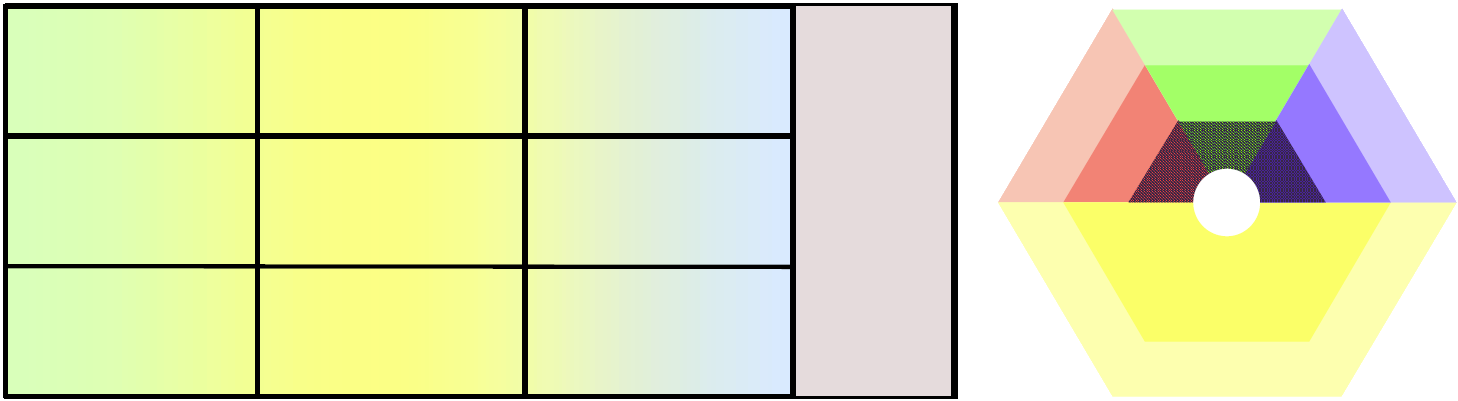
\includegraphics[scale=0.2]{figuras/31}
   	\captionsetup{width=.95\textwidth}
   	\caption{Posición del punto de vista de la contribución conceptualmente y marco del punto de vista \cite{ref9}}
   	\label{figura31}
   \end{figure}
   
   \subsection{Metamodelo\index{Metamodelo}}
   En la figura Figura \ref{metamodelo19} se ilustra el metamodelo del punto de vista de Contribución, en el metamodelo se realza la relación de contribución, esta relación tiene algo a destacar y son las contribuciones positivas y negativas, se apunta a objetivos que aporten de manera positiva y/o negativa hacia los requerimientos que se tratan de diferenciar. \cite{ref9}
   
   \begin{figure}[H]
   	\centering
   	\includegraphics{metamodelos/19}
   	\captionsetup{width=.95\textwidth}
   	\caption{Metamodelo\index{Metamodelo} punto de vista de la contribución \cite{ref9}}
   	\label{metamodelo19}
   \end{figure}
   
   \subsection{Modelo mInstituto}
  La contribución que se espera generar con Minstituto\index{Minstituto}.com en las instituciones educativas es la optimización de sus procesos administrativos generando agilidad y eficiencia en los mismos y logrando un mayor flujo de información influyendo en la agilidad del proceso de toma de decisiones con base en información actualizada y en reportes gerenciales que den una visión global dela organización en diferentes intervalos de tiempo. \\
  
  Tenemos que tener en cuenta que para poder ser ese apoyo organizacional debemos hacer ver nuestro producto como una inversión antes que un costo sin valores agregados y que vamos a estar con ellos realizando el acompañamiento necesario siendo un aliado estratégico en cada una de las etapas del proceso de implementación de un software dentro de una institución, así como en un proceso de capacitación que les permita obtener la mayor utilidad y explotar al máximo su funcionalidad.
  
   \begin{figure}[H]
   	\centering
   	\includegraphics[scale=0.65]{modelos/19}
   	\captionsetup{width=.95\textwidth}
   	\caption{Modelo punto de vista de la contribución: minstituto}
   	\label{modelo19}
   \end{figure}
   
\section{Punto de Vista de Principio\index{Principio}s}
El punto de vista de los principios permite al analista o diseñador modelar los principios que son relevantes para el problema a diseñar, se incluyen los objetivos que motivan a estos principios. Además, las relaciones entre los principios y sus objetivos, pueden ser modelados. Por ejemplo, los principios pueden influir entre sí positiva o negativamente. \cite{ref9}
   
   \begin{table}[H]
   	\centering
   	\begin{tabular}{p{3.7cm}p{8cm}}
   		\hline
   		\rowcolor[HTML]{0073a1}
   		{\color[HTML]{FFFFFF} \textbf{Nombre}} & {\color[HTML]{FFFFFF} \textbf{Vista de Principio\index{Principio}s}} \\
   		\hline
   		\textbf{Stakeholder\index{Stakeholder}s} & Stakeholder\index{Stakeholder}s, administradores de empresas, arquitectos TIC\index{TIC}, analistas de negocios, Analistas de requerimientos \\
   		\textbf{Preocupaciones} & Misión de arquitectura, estrategia y táctica, motivación \\
   		\textbf{Propósito} & Diseñar\index{Diseñar}, decidir \\
   		\textbf{Nivel de Abstracción\index{Abstracción}} & Coherencia\index{Coherencia}, detalle \\
   		\textbf{Capa} & Capa de negocio, tecnología \\
   		\textbf{Aspectos} & Motivación \\
   		\bottomrule
   	\end{tabular}
   	\captionsetup{width=.95\textwidth}
   	\caption{Descripción punto de vista de los principios \cite{ref9}}
   	\label{tabla23}
   \end{table}
   
   \begin{figure}[H]
   	\centering
   	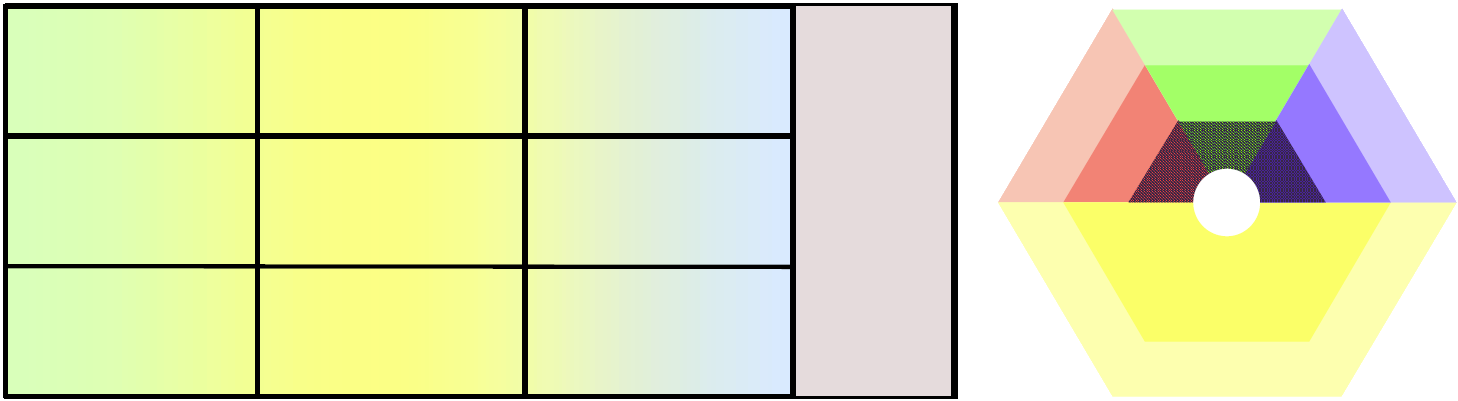
\includegraphics[scale=0.2]{figuras/32}
   	\captionsetup{width=.95\textwidth}
   	\caption{Posición del punto de vista de los principios conceptualmente y marco del punto de vista \cite{ref9}}
   	\label{figura32}
   \end{figure}
   
   \subsection{Metamodelo\index{Metamodelo}}
   En la figura Figura \ref{metamodelo20} se ilustra el metamodelo del punto de vista de Principio\index{Principio}s, los principios son características que le dan caracterización,matizan o resaltan a la organización en los objetivos, le asocia adjetivos que apuntalan la naturaleza de la organización. \cite{ref9}
   
   \begin{figure}[H]
   	\centering
   	\includegraphics{metamodelos/20}
   	\captionsetup{width=.95\textwidth}
   	\caption{Metamodelo\index{Metamodelo} punto de vista de los principios \cite{ref9}}
   	\label{metamodelo20}
   \end{figure}
   
   \subsection{Modelo mInstituto}
   Cuando hablamos de principios de nuestra organización es importante resaltar que debemos tener un sistema que cumpla con los estándares de confidencialidad: Salvaguardar\index{Salvaguardar} la información. Integridad\index{Integridad}: Que los datos sean consistentes y suplan las necesidades para la toma de decisiones correctas. Disponibilidad: disponer de un gestor que le brinde a cada usuario los datos autorizados y que de igual manera estén siempre visibles en el momento en que los clientes los quieran consultar. Innovación: Es importante resaltar que nuestra empresa y sus productos deben estar en un constante cambio para estar al día con las nuevas propuestas, tecnologías y exigencias del mercado.
   
   \begin{figure}[H]
   	\centering
   	\includegraphics[scale=0.6]{modelos/20}
   	\captionsetup{width=.95\textwidth}
   	\caption{Modelo punto de vista de los principios: minstituto}
   	\label{modelo20}
   \end{figure}
   
\section{Punto de Vista de Realización de Requerimientos}
El punto de vista de realización de requerimientos permite al diseñador modelar la realización de los requerimientos para los elementos base o core, tales como los actores de negocios, servicios de negocios, procesos de negocios, servicios de aplicaciones, componentes de la aplicación, etc. Por lo general, los requisitos son el resultado del punto de vista de refinamiento del objetivo. Además, este punto de vista se puede usar para refinar los requisitos en requisitos más detallados. La relación de agregación se usa para este propósito. \cite{ref9}
   
   \begin{table}[H]
   	\centering
   	\begin{tabular}{p{3.7cm}p{8cm}}
   		\hline
   		\rowcolor[HTML]{0073a1}
   		{\color[HTML]{FFFFFF} \textbf{Nombre}} & {\color[HTML]{FFFFFF} \textbf{Realización de Requerimientos}} \\
   		\hline
   		\textbf{Stakeholder\index{Stakeholder}s} & Stakeholder\index{Stakeholder}s, administradores de empresas, arquitectos TIC\index{TIC}, analistas de negocios, Analistas de requerimientos \\
   		\textbf{Preocupaciones} & Misión de arquitectura, estrategia y táctica, motivación \\
   		\textbf{Propósito} & Diseñar\index{Diseñar}, decidir \\
   		\textbf{Nivel de Abstracción\index{Abstracción}} & Coherencia\index{Coherencia}, detalle \\
   		\textbf{Capa} & Capa de Aplicación\index{Aplicación}, tecnología \\
   		\textbf{Aspectos} & Motivación \\
   		\bottomrule
   	\end{tabular}
   	\captionsetup{width=.95\textwidth}
   	\caption{Descripción punto de vista de realización de requerimientos \cite{ref9}}
   	\label{tabla24}
   \end{table}
   
   \begin{figure}[H]
   	\centering
   	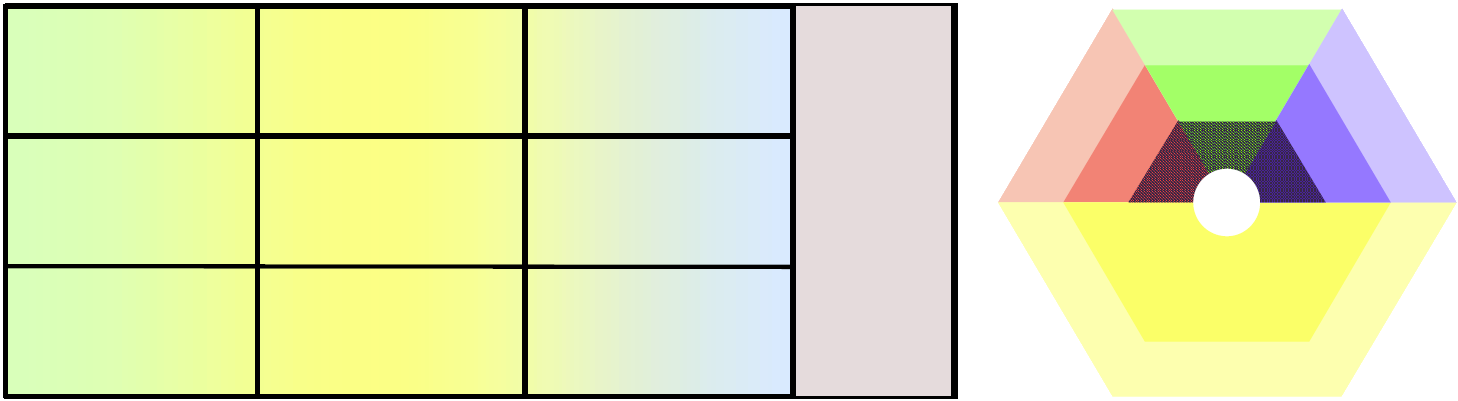
\includegraphics[scale=0.2]{figuras/33}
   	\captionsetup{width=.95\textwidth}
   	\caption{Posición del punto de vista de realización de requerimientos conceptualmente y marco del punto de vista \cite{ref9}}
   	\label{figura33}
   \end{figure}
   
   \subsection{Metamodelo\index{Metamodelo}}
   En la Figura \ref{metamodelo21} se ilustra el metamodelo del punto de vista de Realización de Requerimientos, la realización de requerimientos tiene un vocabulario que se aleja del negocio y pone más en términos de requerimiento, se toma el objetivo y se desagrega; el lenguaje utilizado es un lenguaje apropiado para entenderlo. \cite{ref9}
   
   \begin{figure}[H]
   	\centering
   	\includegraphics{metamodelos/21}
   	\captionsetup{width=.95\textwidth}
   	\caption{Metamodelo\index{Metamodelo} punto de vista de realización de requerimientos \cite{ref9}}
   	\label{metamodelo21}
   \end{figure}
   
   \subsection{Modelo mInstituto}
   Para proveer soluciones tecnológicas que permitan optimizar la gestión de la información en las instituciones educativas debemos conocer la dinámica de estas, identificar sus necesidades y dificultades a las que se enfrentan cada día al no tener una solución tecnológica que les permita disponer de información actualizada y precisa de la gestión de la institución, se debe concientizar al cliente de que la solución tecnológica representa una inversión y no un costo y debe ser un entorno amigable de fácil navegación. \\
   
   Con respecto a las licencias debemos alinearnos con el modelo de requerimientos ofrecido a los clientes.

   \begin{figure}[H]
   	\centering
   	\includegraphics[scale=0.65]{modelos/21}
   	\captionsetup{width=.95\textwidth}
   	\caption{Modelo punto de vista de realización de requerimientos: minstituto}
   	\label{modelo21}
   \end{figure}
   
\section{Punto de Vista de Motivación}
El punto de vista de la motivación permite al diseñador o analista modelar el aspecto motivacional, sin centrarse en ciertos elementos dentro de este aspecto. Por ejemplo, este punto de vista se puede utilizar para presentar una visión completa o parcial del aspecto de motivación por parte de los stakeholders, los principales objetivos, los principios que se aplican, y los requerimientos principales de los servicios, procesos, aplicaciones y objetos. \cite{ref9}

   \begin{table}[H]
   	\centering
   	\begin{tabular}{p{3.7cm}p{8cm}}
   		\hline
   		\rowcolor[HTML]{0073a1}
   		{\color[HTML]{FFFFFF} \textbf{Nombre}} & {\color[HTML]{FFFFFF} \textbf{Motivación}} \\
   		\hline
   		\textbf{Stakeholder\index{Stakeholder}s} & Stakeholder\index{Stakeholder}s, administradores de empresas, arquitectos TIC\index{TIC}, analistas de negocios, Analistas de requerimientos \\
   		\textbf{Preocupaciones} & Misión de arquitectura, estrategia y táctica, motivación \\
   		\textbf{Propósito} & Diseñar\index{Diseñar}, decidir \\
   		\textbf{Nivel de Abstracción\index{Abstracción}} & Coherencia\index{Coherencia}, detalle \\
   		\textbf{Capa} & Capa de Aplicación\index{Aplicación}, tecnología \\
   		\textbf{Aspectos} & Motivación \\
   		\bottomrule
   	\end{tabular}
   	\captionsetup{width=.95\textwidth}
   	\caption{Descripción punto de vista de la motivación \cite{ref9}}
   	\label{tabla25}
   \end{table}
   
   \begin{figure}[H]
   	\centering
   	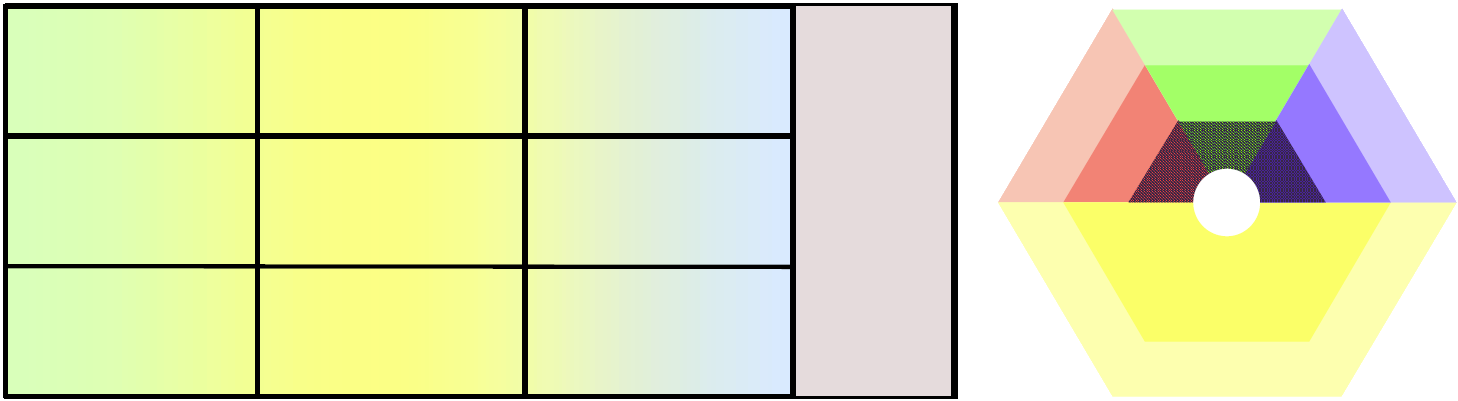
\includegraphics[scale=0.2]{figuras/34.png}
   	\captionsetup{width=.95\textwidth}
   	\caption{Posición del punto de vista de la motivación conceptualmente y marco del punto de vista \cite{ref9}}
   	\label{figura34}
   \end{figure}
   
   \subsection{Metamodelo\index{Metamodelo}}
   En la Figura \ref{metamodelo22} se ilustra el metamodelo del punto de vista de Motivación, donde el punto angular es el participante que tiene una valoración y cuenta con un objetivo clave el cual se relaciona con los requerimientos, al participante se le asocia el manejador que es una asociación es parecida a un objetivo pero es propia del participante, se puede decir que es un objetivo del participante. Con este punto de vista se muestra la esencia de la parte motivacional. De esto se puede decir que el punto de vista se centra en el participante lo que él hace, los requerimientos que el genera, en la valoración que el produce, la asociación con el objetivo organizacional y el manejo que tiene con respecto al negocio. \cite{ref9}
   
   \begin{figure}[H]
   	\centering
   	\includegraphics{metamodelos/22}
   	\captionsetup{width=.95\textwidth}
   	\caption{Metamodelo\index{Metamodelo} punto de vista de la motivación \cite{ref9}}
   	\label{metamodelo22}
   \end{figure}
   
   \subsection{Modelo mInstituto}
   Como principal motivación del proyecto a desarrollar por parte de nuestra organización es tener esa participación en el mercado de las instituciones educativas, que nos permita crecer como organización y como miembros de la misma. Sin embargo, para lograr ese objetivo es necesario que nuestro software esté en capacidad de soportar la dinámica de negocio de nuestros clientes, manteniendo la confidencialidad y disponibilidad de su información.
   
   \begin{figure}[H]
   	\centering
   	\includegraphics[scale=0.6]{modelos/22}
   	\captionsetup{width=.95\textwidth}
   	\caption{Modelo punto de vista de la motivación: minstituto}
   	\label{modelo22}
   \end{figure}